\begin{frame}
%\note[item]<100>{As músicas automáticas foram gravadas com um piano MIDI}
%\note[item]<100>{As músicas anotadas foram anotadas manulmente, no nível de nota no rachmaninoff e pulso para as sinfonias}
%\note[item]<100>{7 Performances adicionais foram coletadas sem anotação, apenas para serem processadas de forma automática. Com exceção das que já tem 22 (7 foram escolhidas aleatoriamente dentre elas, sem repetir o performer)}
%\note[item]<100>{dizer que existem duas musicas orquestrais, dificuldade maior}
%\note[item]<100>{dizer que foi obtido mais de uma gravação da mesma musica}
  \frametitle{Descrição dos dados}
  \pause
  \begin{center}
    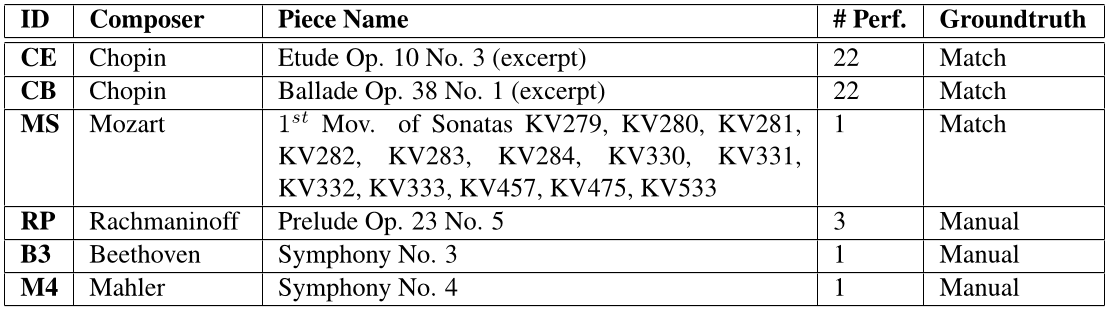
\includegraphics[width=\textwidth]{src/img/1-Table1-1.png}
  \end{center}
\end{frame}

\begin{frame}
  \frametitle{Rastreamento padrão baseado em representação simbólica musical}
  Abordagem baseada no algoritmo \emph{Dynamic Time Warping (DTW)} com algumas extensões:\pause
%\note[item]<100>{  que possibilitam a aplicação em rastreamento online. [artigo 10]}
  \begin{itemize}
    \item O caminho é computado de maneira incremental\\\pause
    \item A complexidade é reduzida para ser linear no tamanho da entrada\pause
    \item Utiliza a estratégia \emph{backward-forward}
%\note[item]<100>{reconsidera decisoes passadas, aumenta robustez [artigo 4]}
%\note[item]<100>{ aumenta a habilidade de o algoritmo lidar com diferencas no Andamento [artigo 3] }
  \end{itemize}
\end{frame}

\begin{frame}
  \frametitle{Rastreamento padrão baseado em representação simbólica musical}
  %\note[item]<100>{ Para ser possível o tracking é necessário...}
  Precisamos de uma representação da partitura\pause
  \begin{itemize}
    \item Síntese MIDI -> áudio\\\pause
    \item Alinhamento áudio-áudio, agora com a informação temporal de cada nota\pause
  \end{itemize}
  Nesse artigo, é usado uma mistura de características cromáticas e de início de nota \emph{(semi-tone onset)} e o algoritmo explicado anteriormente
\end{frame}

\begin{frame}
  \frametitle{Resultados utilizando o rastreamento padrão}
  \begin{center}
    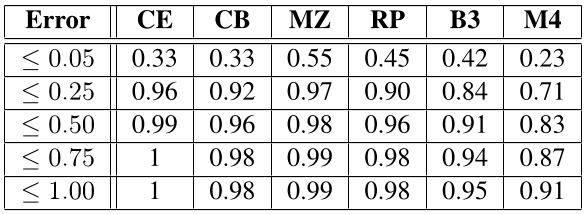
\includegraphics[width=0.8\textwidth]{src/img/1-Table2-1.png}
  \end{center}
  \pause
  \begin{itemize}
    \item Funciona bem para peças em piano\\\pause
    \item Não funciona bem para peças orquestrais
    %\note[item]<100>{É fácil sintetizar piano mas é muito mais complexo para orquestras}
  \end{itemize}
\end{frame}

\begin{frame}
  \frametitle{Rastreamento utilizando uma performance como referência}
  O rastreamento padrão funciona bem mas ganhamos algumas vantagens ao utilizar uma performance real como referência:\pause
  \begin{itemize}
    \item Melhor qualidade\pause
    \item Características mais próximas da performance ao vivo que queremos rastrear\pause
    \item Maior similaridade sonora, principalmente em peças orquestradas\pause
    \item Informações detalhadas de andamento, dinâmica e articulação
  \end{itemize}
\end{frame}

\begin{frame}
  \frametitle{Rastreamento utilizando uma performance como referência}
  Porém, temos uma grande desvantagem:\pause
  \begin{itemize}
    \item A informação temporal das notas é inexistente\pause
  \end{itemize}
  Assim, precisaremos calcular esta informação para seguir essa abordagem. \pause Nesse artigo, isso será feito de forma automática
\end{frame}

\againframe<1>{figura1}

\begin{frame}
  \frametitle{Alinhamento off-line}
  \begin{itemize}
    \item Espera-se que o aumento na qualidade das características supere o erro introduzido por esta etapa\pause
    \item Aqui, usamos o algoritmo já citado, com a única diferença de que, no final, computamos o caminho contrário, como se faz no DTW padrão.
    %\note[item]<100>{ É claro que podemos usar qualquer algoritmo de alinhamento}
  \end{itemize}
  Assim, temos resultados melhores que o caso online.
\end{frame}

\begin{frame}
  \frametitle{Comparação dos resultados}

  \begin{figure}[!tbp]
    \centering
    \begin{minipage}[b]{0.45\textwidth}
      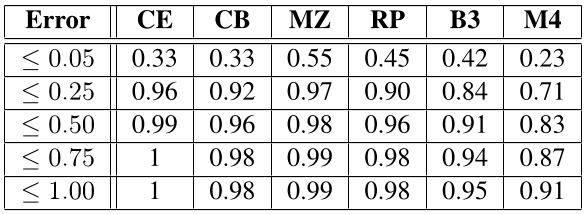
\includegraphics[width=\textwidth]{src/img/1-Table2-1.png}
      \caption*{Rastreamento padrão}
    \end{minipage}
    \hfill
    \begin{minipage}[b]{0.45\textwidth}
      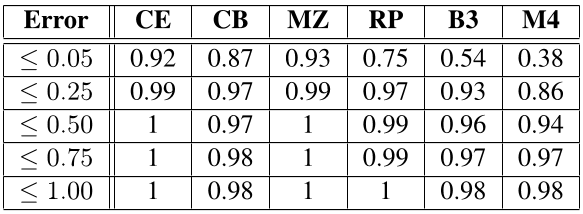
\includegraphics[width=\textwidth]{src/img/1-Table3-1.png}
      \caption*{Alinhamento off-line}
    \end{minipage}
  \end{figure}
\end{frame}

\begin{frame}
  \frametitle{Rastreamento baseado em uma performance alinhada}
  Agora, utilizando a performance já alinhada, utilizamos o mesmo algoritmo de rastreamento para as outras performances.
  Estes são os resultados:
  \begin{figure}[!ht]
    \centering
    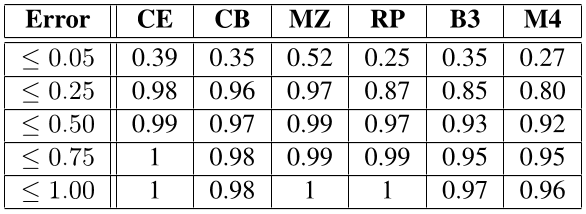
\includegraphics[width=0.7\textwidth]{src/img/3-Table4-1.png}
    \caption*{Rastreamento on-line baseado em uma performance alinhada off-line}
  \end{figure}
\end{frame}

\begin{frame}
  \frametitle{Rastreamento baseado em uma performance alinhada}
  \begin{itemize}
    \item Melhoria nas peças orquestradas\pause
    \item Resultados se mostraram instáveis - algumas performances são mais similares entre si do que com a usada como referência \pause %Infelizmente
    \item Resultados mostraram que algumas partes da peça tiveram erros frequentemente \pause %A peça é difícil mesmo
    \item Utilizando diferentes performances como referência, alguns erros só apareciam em uma ou duas delas \pause
  \end{itemize}
  Isto levou à ideia de combinar o alinhamento de várias performances para diminuir estes erros.
\end{frame}

\begin{frame}[label=figura2]
  \frametitle{Rastreamento baseado em várias performances alinhadas}
  \begin{figure}[!ht]
    \centering
    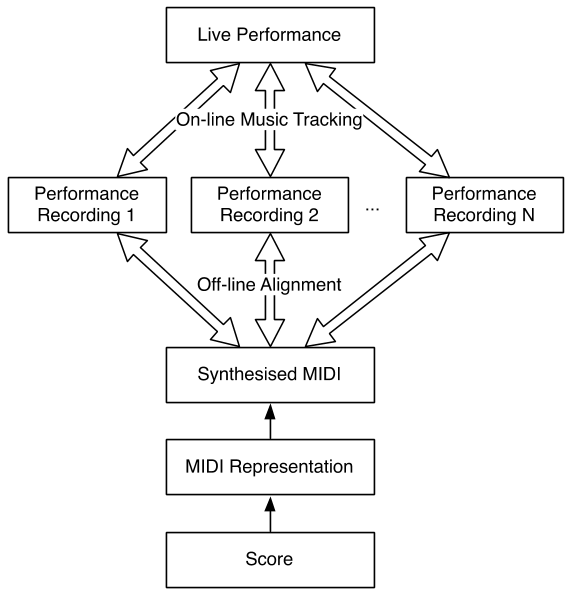
\includegraphics[height=0.7\textheight]{src/img/2-Figure2-1.png}
    \caption*{Rastreamento multi-agente baseado em várias performances alinhadas off-line}
  \end{figure}
\end{frame}

\begin{frame}
  \frametitle{Rastreamento baseado em múltiplas performances}
  \begin{itemize}
    \item Várias anotações alinhadas são usadas em paralelo no rastreamento\pause
    \item Utilizamos a mediana \pause %Explicar o porquê
    \item Mais estabilidade em aplicações práticas \pause
    \item Foram utilizadas 7 performances\pause 
%\note[item]<100>{explicar tradeoff robustez x tempo de computação}
  \end{itemize}
\end{frame}
